\chapter{Eksperimentalna analiza rada sistema}

Krerani sistem napravljen je od nekoliko podsistema koji su usklađeni u jednu cjelinu.

Prvi podsistem je osvjetljenje, rpikazano na slici \ref{fig:Slika_osvjetljenje}, postignuto pojedinačnim LED diodama, te LED svjetlima iz novogodišnjeg ukrasa. Uključuje se i isključuje po korisnikovoj želji uz pomoć aplikacije. 

\begin{figure}[h!]
  \centering
  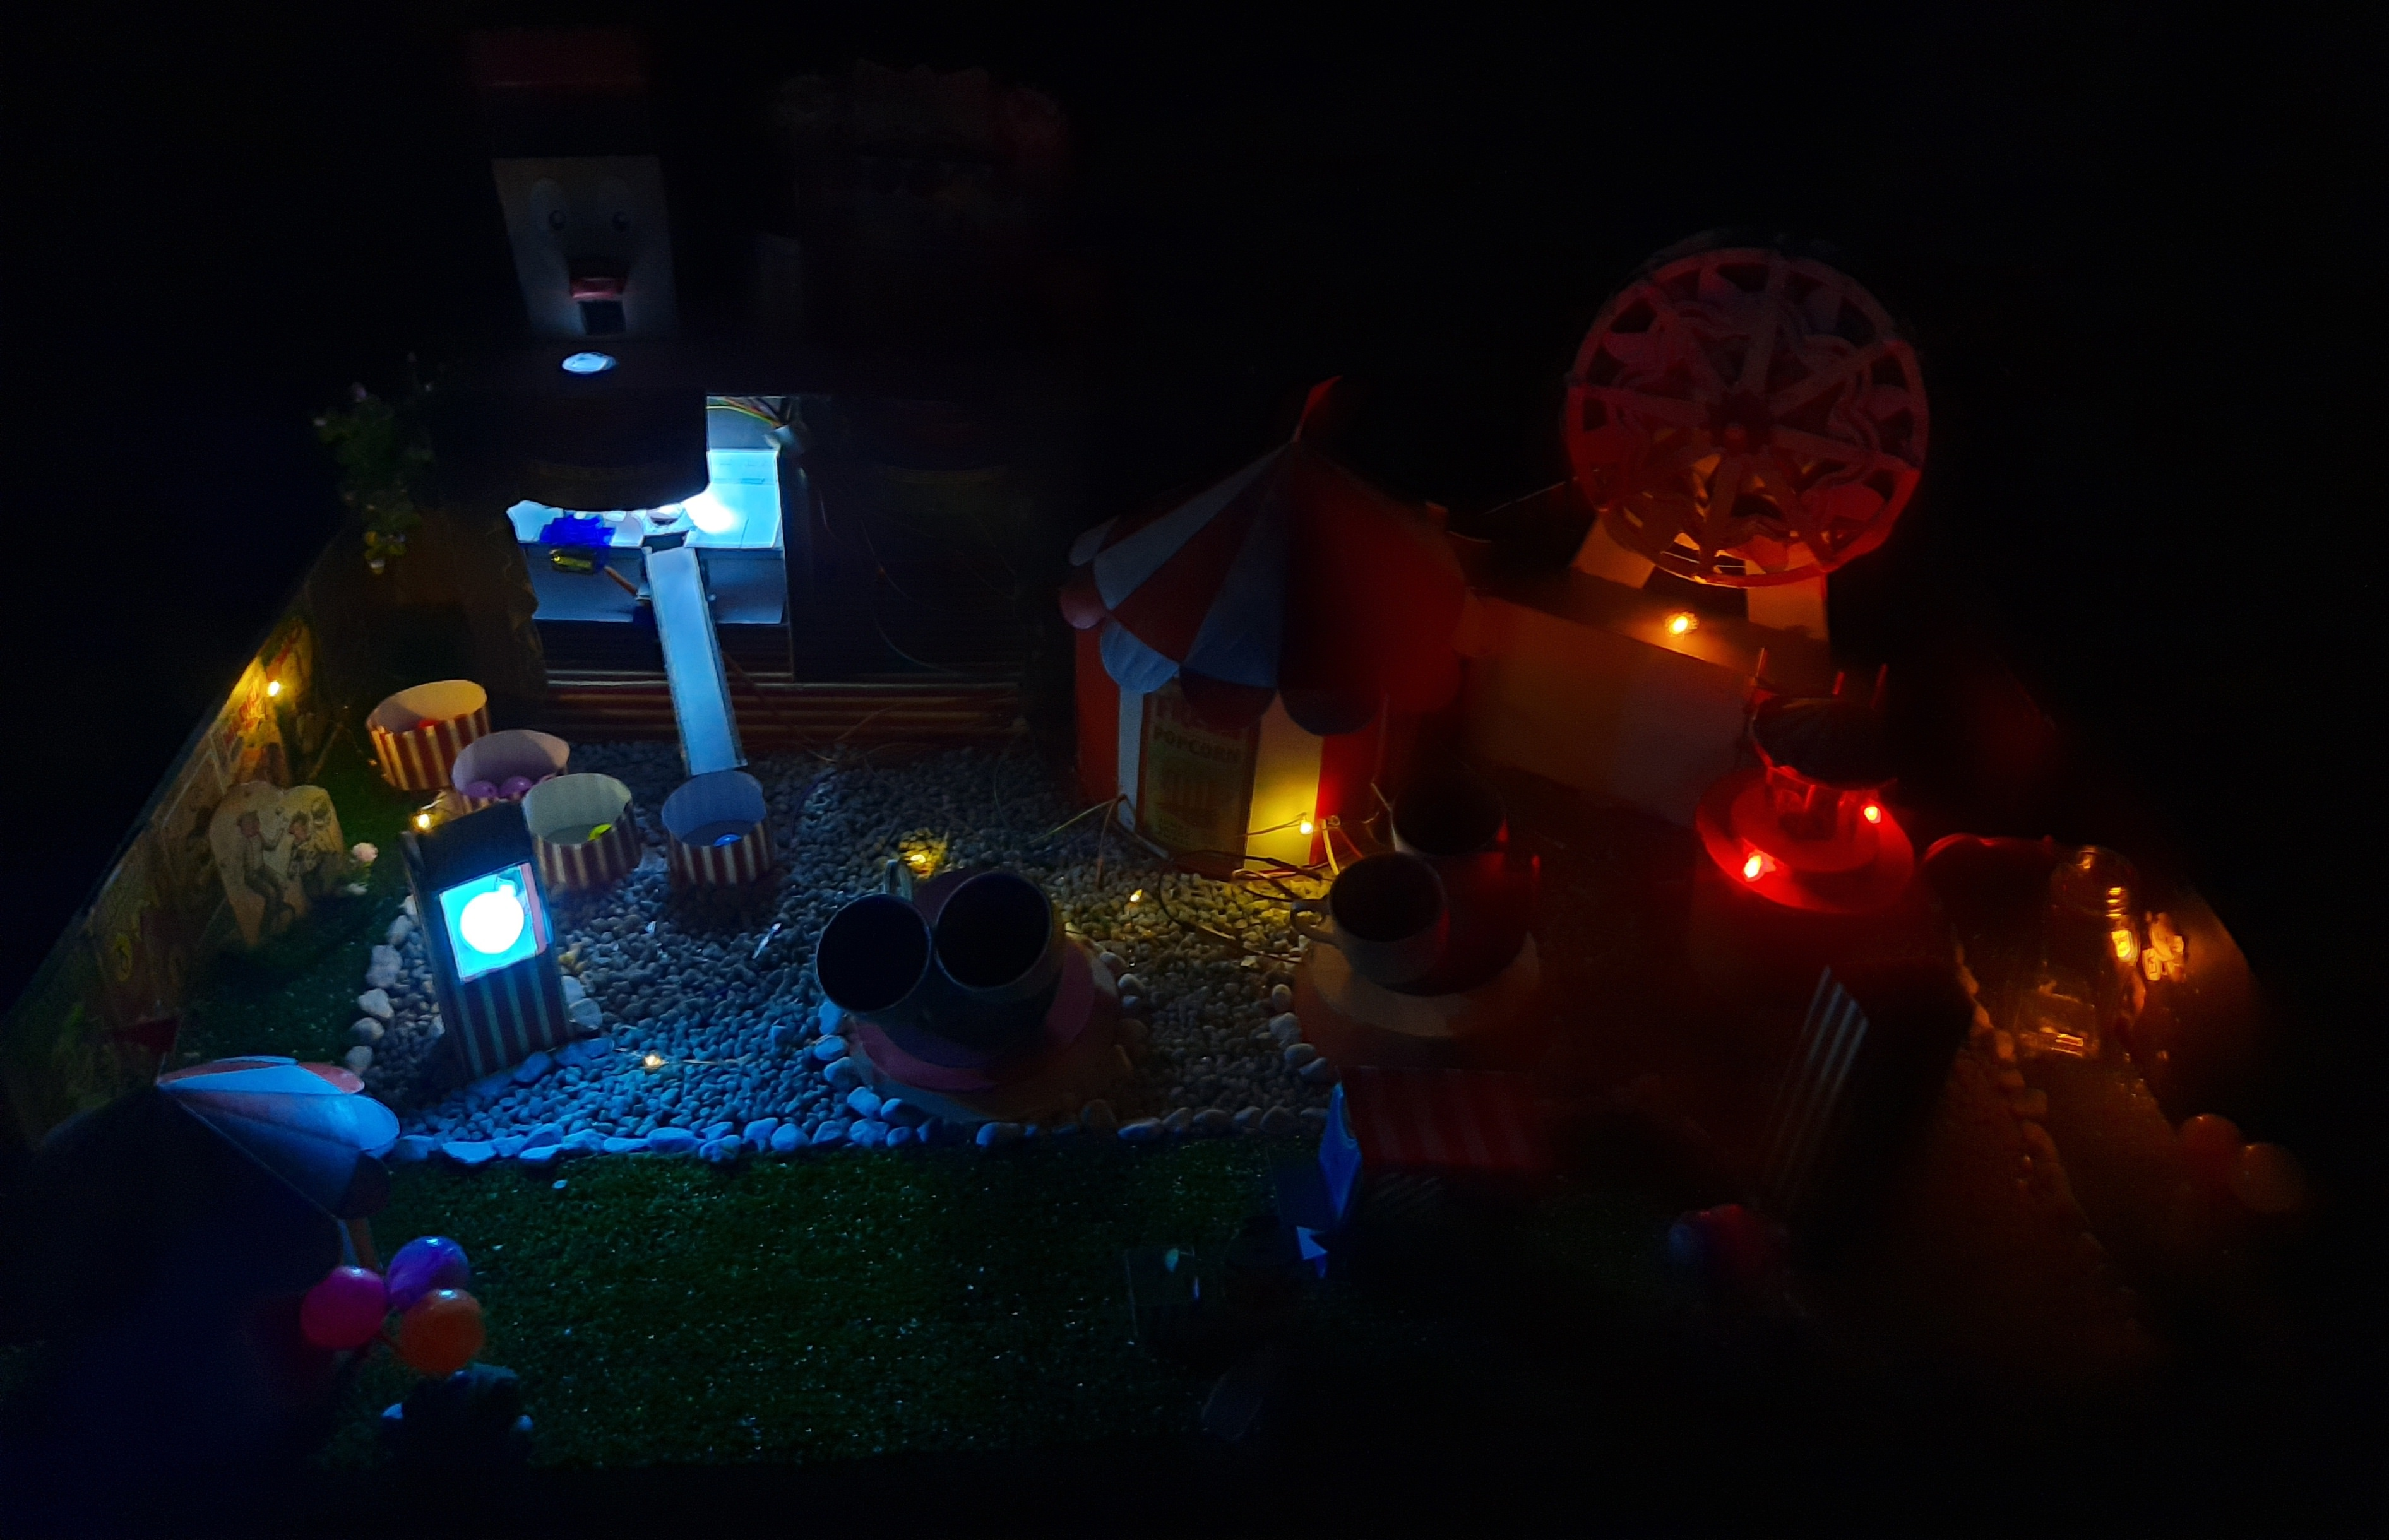
\includegraphics[width=0.7\textwidth]{svjetla}
  \caption{Osvjetljenje sistema}
  \label{fig:Slika_osvjetljenje}
\end{figure}

Drugi podsistem je igra, prikazana izbliza na slici \ref{fig:Slika_pod1}, u kojoj korisnik pogađa boju loptice koja izađe iz aparata. Prvo pusti lopticu da uđe u podsistem, odabere na mobitelu da će igrati igru, te onda pogađa boju loptice pritiskom push buttona, koji je smješten u dizajn igre ''pogodi balon'', koja često bude u zabavnim parkovima. Ako pogodi boju, zasvijetli zelena dioda, a ako promaši, zasvijeli crvena. Boja se čita senzorom za boju, a servo motorima se loptice prebacuju u određenu posudu. U posudama su loptice sortirane po boji.

Treći podsistem je vračara, također vidljiva na slici \ref{fig:Slika_pod1}, čija RGB dioda se uključuje se i isključuje po korisnikovoj želji uz pomoć aplikacije.

\begin{figure}[h!]
  \centering
  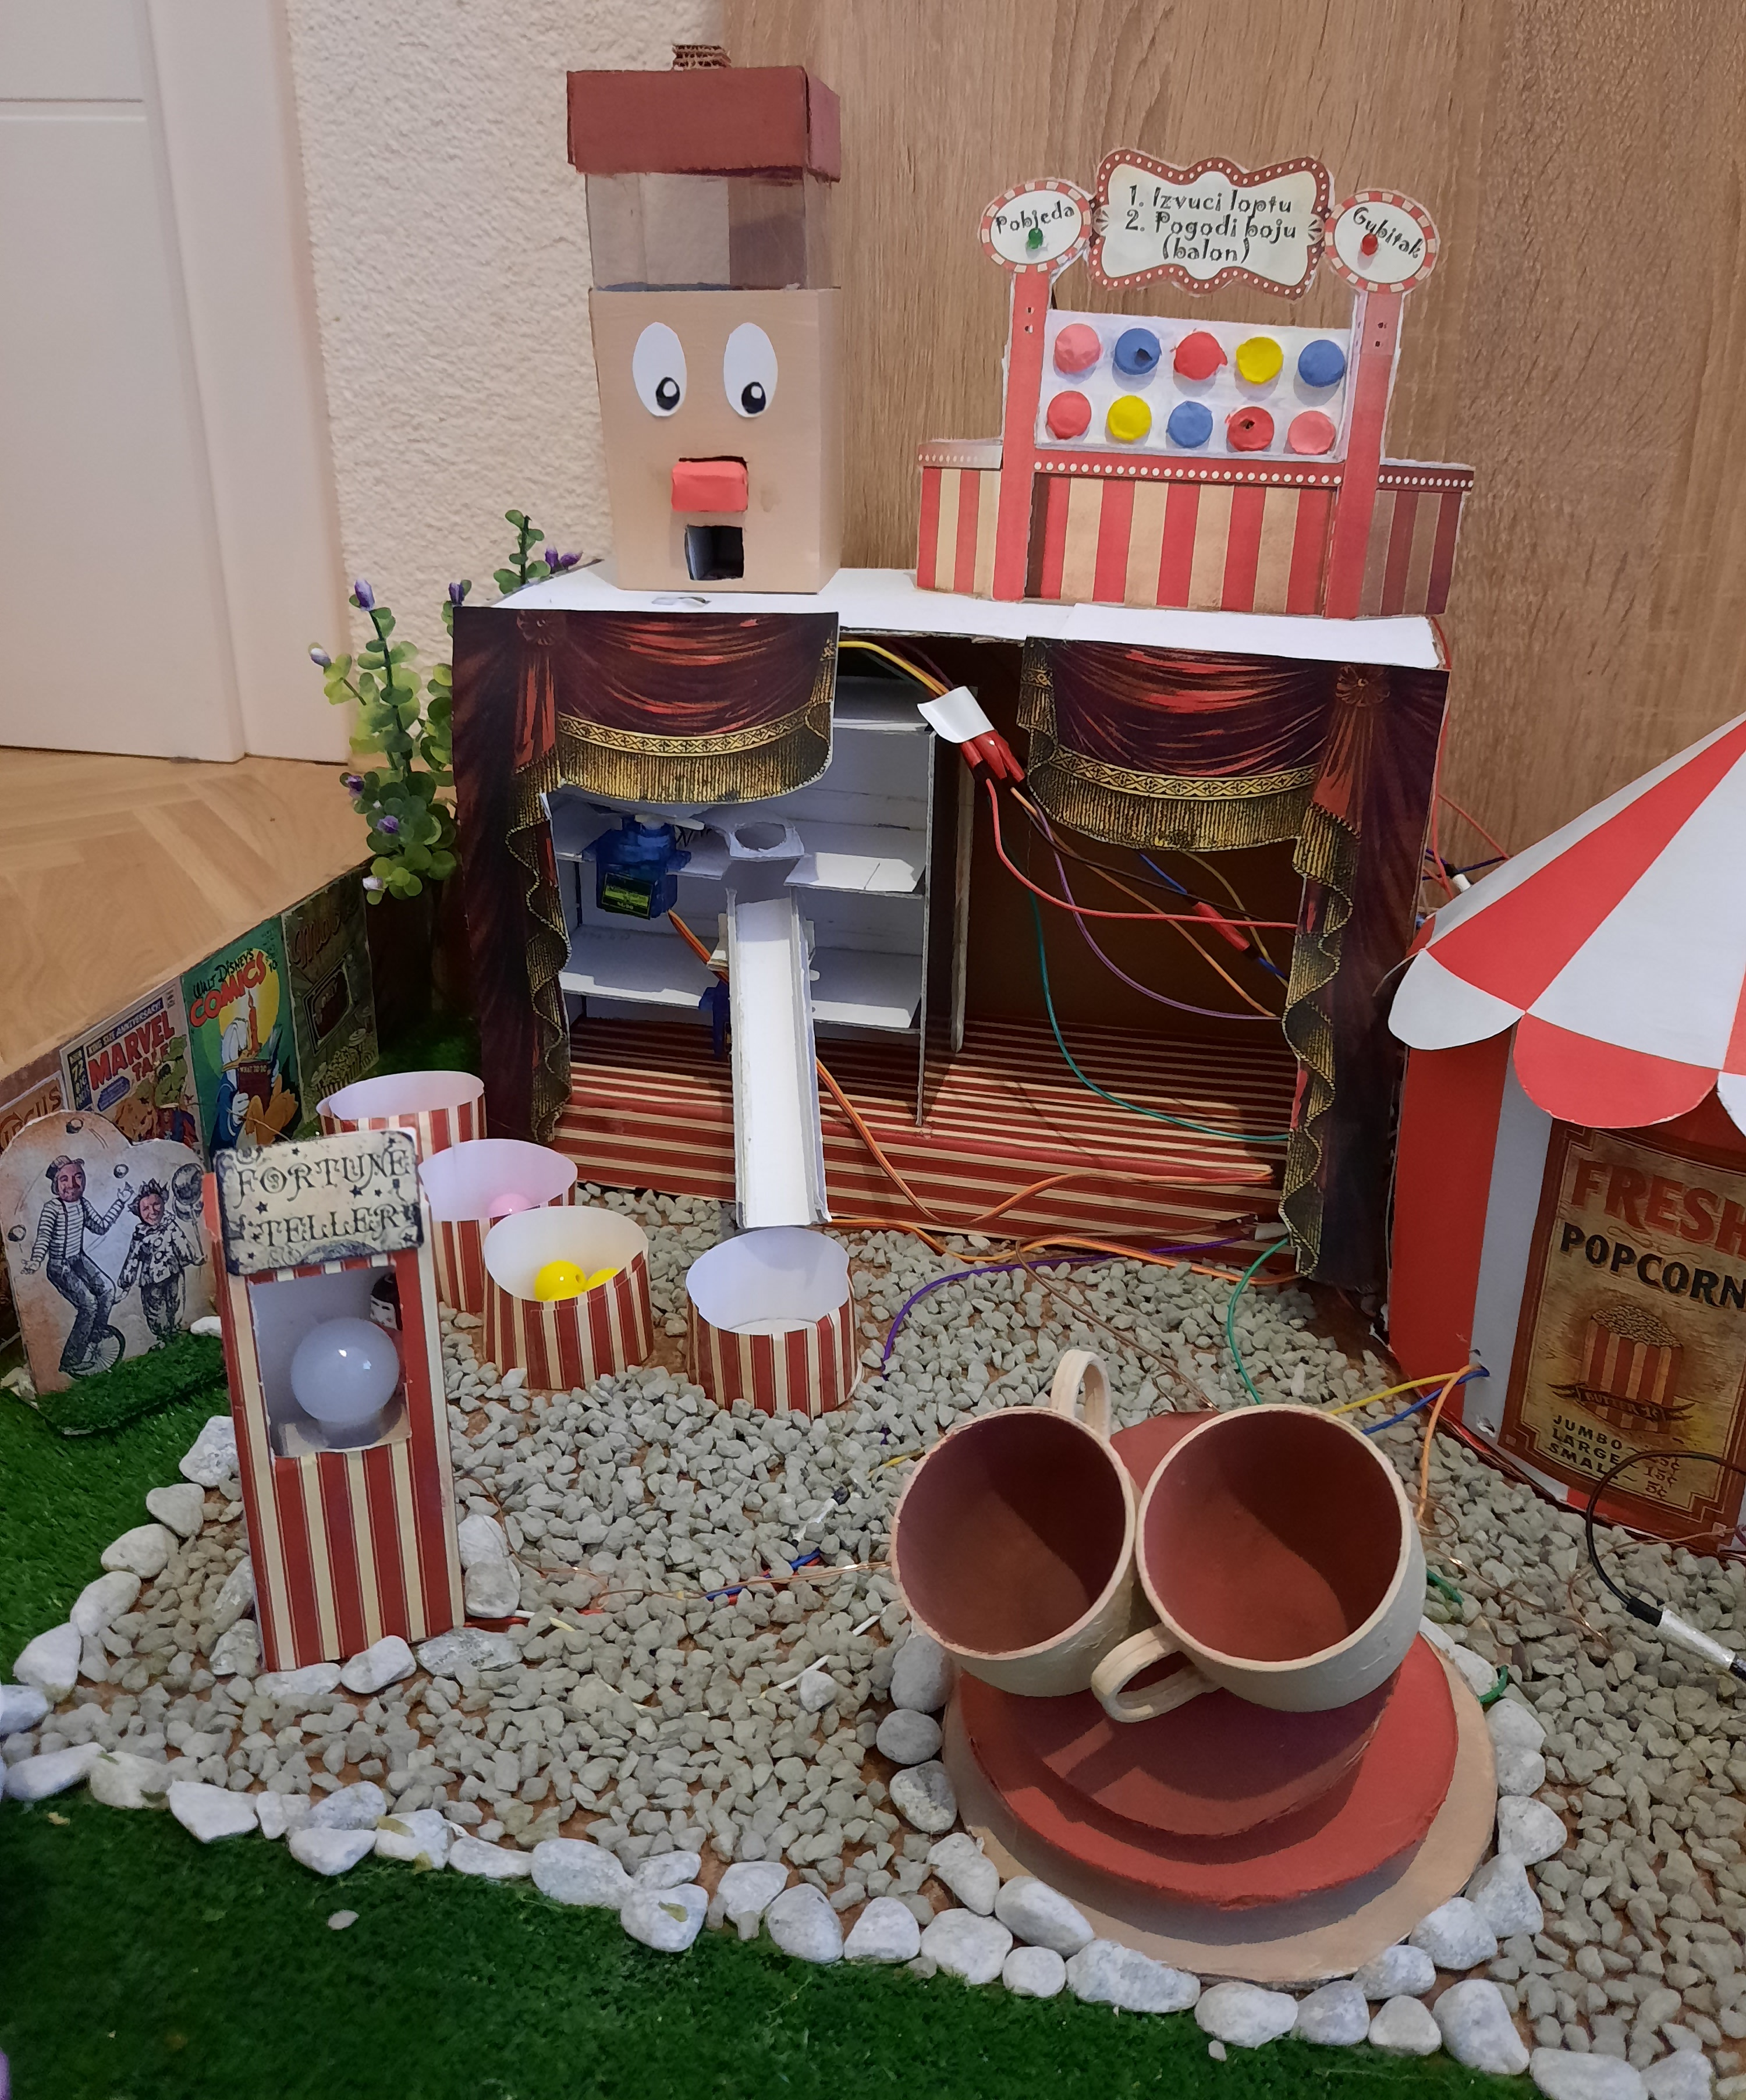
\includegraphics[width=0.5\textwidth]{pod1}
  \caption{Podsistemi igra i vračara}
  \label{fig:Slika_pod1}
\end{figure}

Četvrti podsistem je karusel, odnosno vrtuljak sa konjićima. Napravljen je od kartona po šablonu s Interneta. U sebi sadrži DC motor sa zupčanicima koji usporava njegovo okretanje kako ne bi bio prebrz. Pokreće se i zaustavlja po korisnikovoj želji uz pomoć aplikacije.

Peti podsistem je vrtuljak. Napravljen je od jako detaljnog šablona koji je preuzet s Interneta i modificiran kako bi odgovarao sistemu. Ima sjedala koja se mogu pomjerati. U njemu se nalazi jači DC motor, od 12 V, pošto ga slabiji ne mogu pokrenuti. Pokreće se i zaustavlja po korisnikovoj želji uz pomoć aplikacije.

Šesti podsistem su šoljice, koje se vrte uz pomoć DC motora ispod njih. Pokreću se i zaustavljaju po korisnikovoj želji uz pomoć aplikacije. Kako bi svi DC motori imali dovoljno snage da se pokrenu, samo za njih je osiguran ulazni napon od 6 baterija po 1,5 V, koji je puno bolji za DC motore od standardnih baterija od 9 V. 

\begin{figure}[h!]
  \centering
  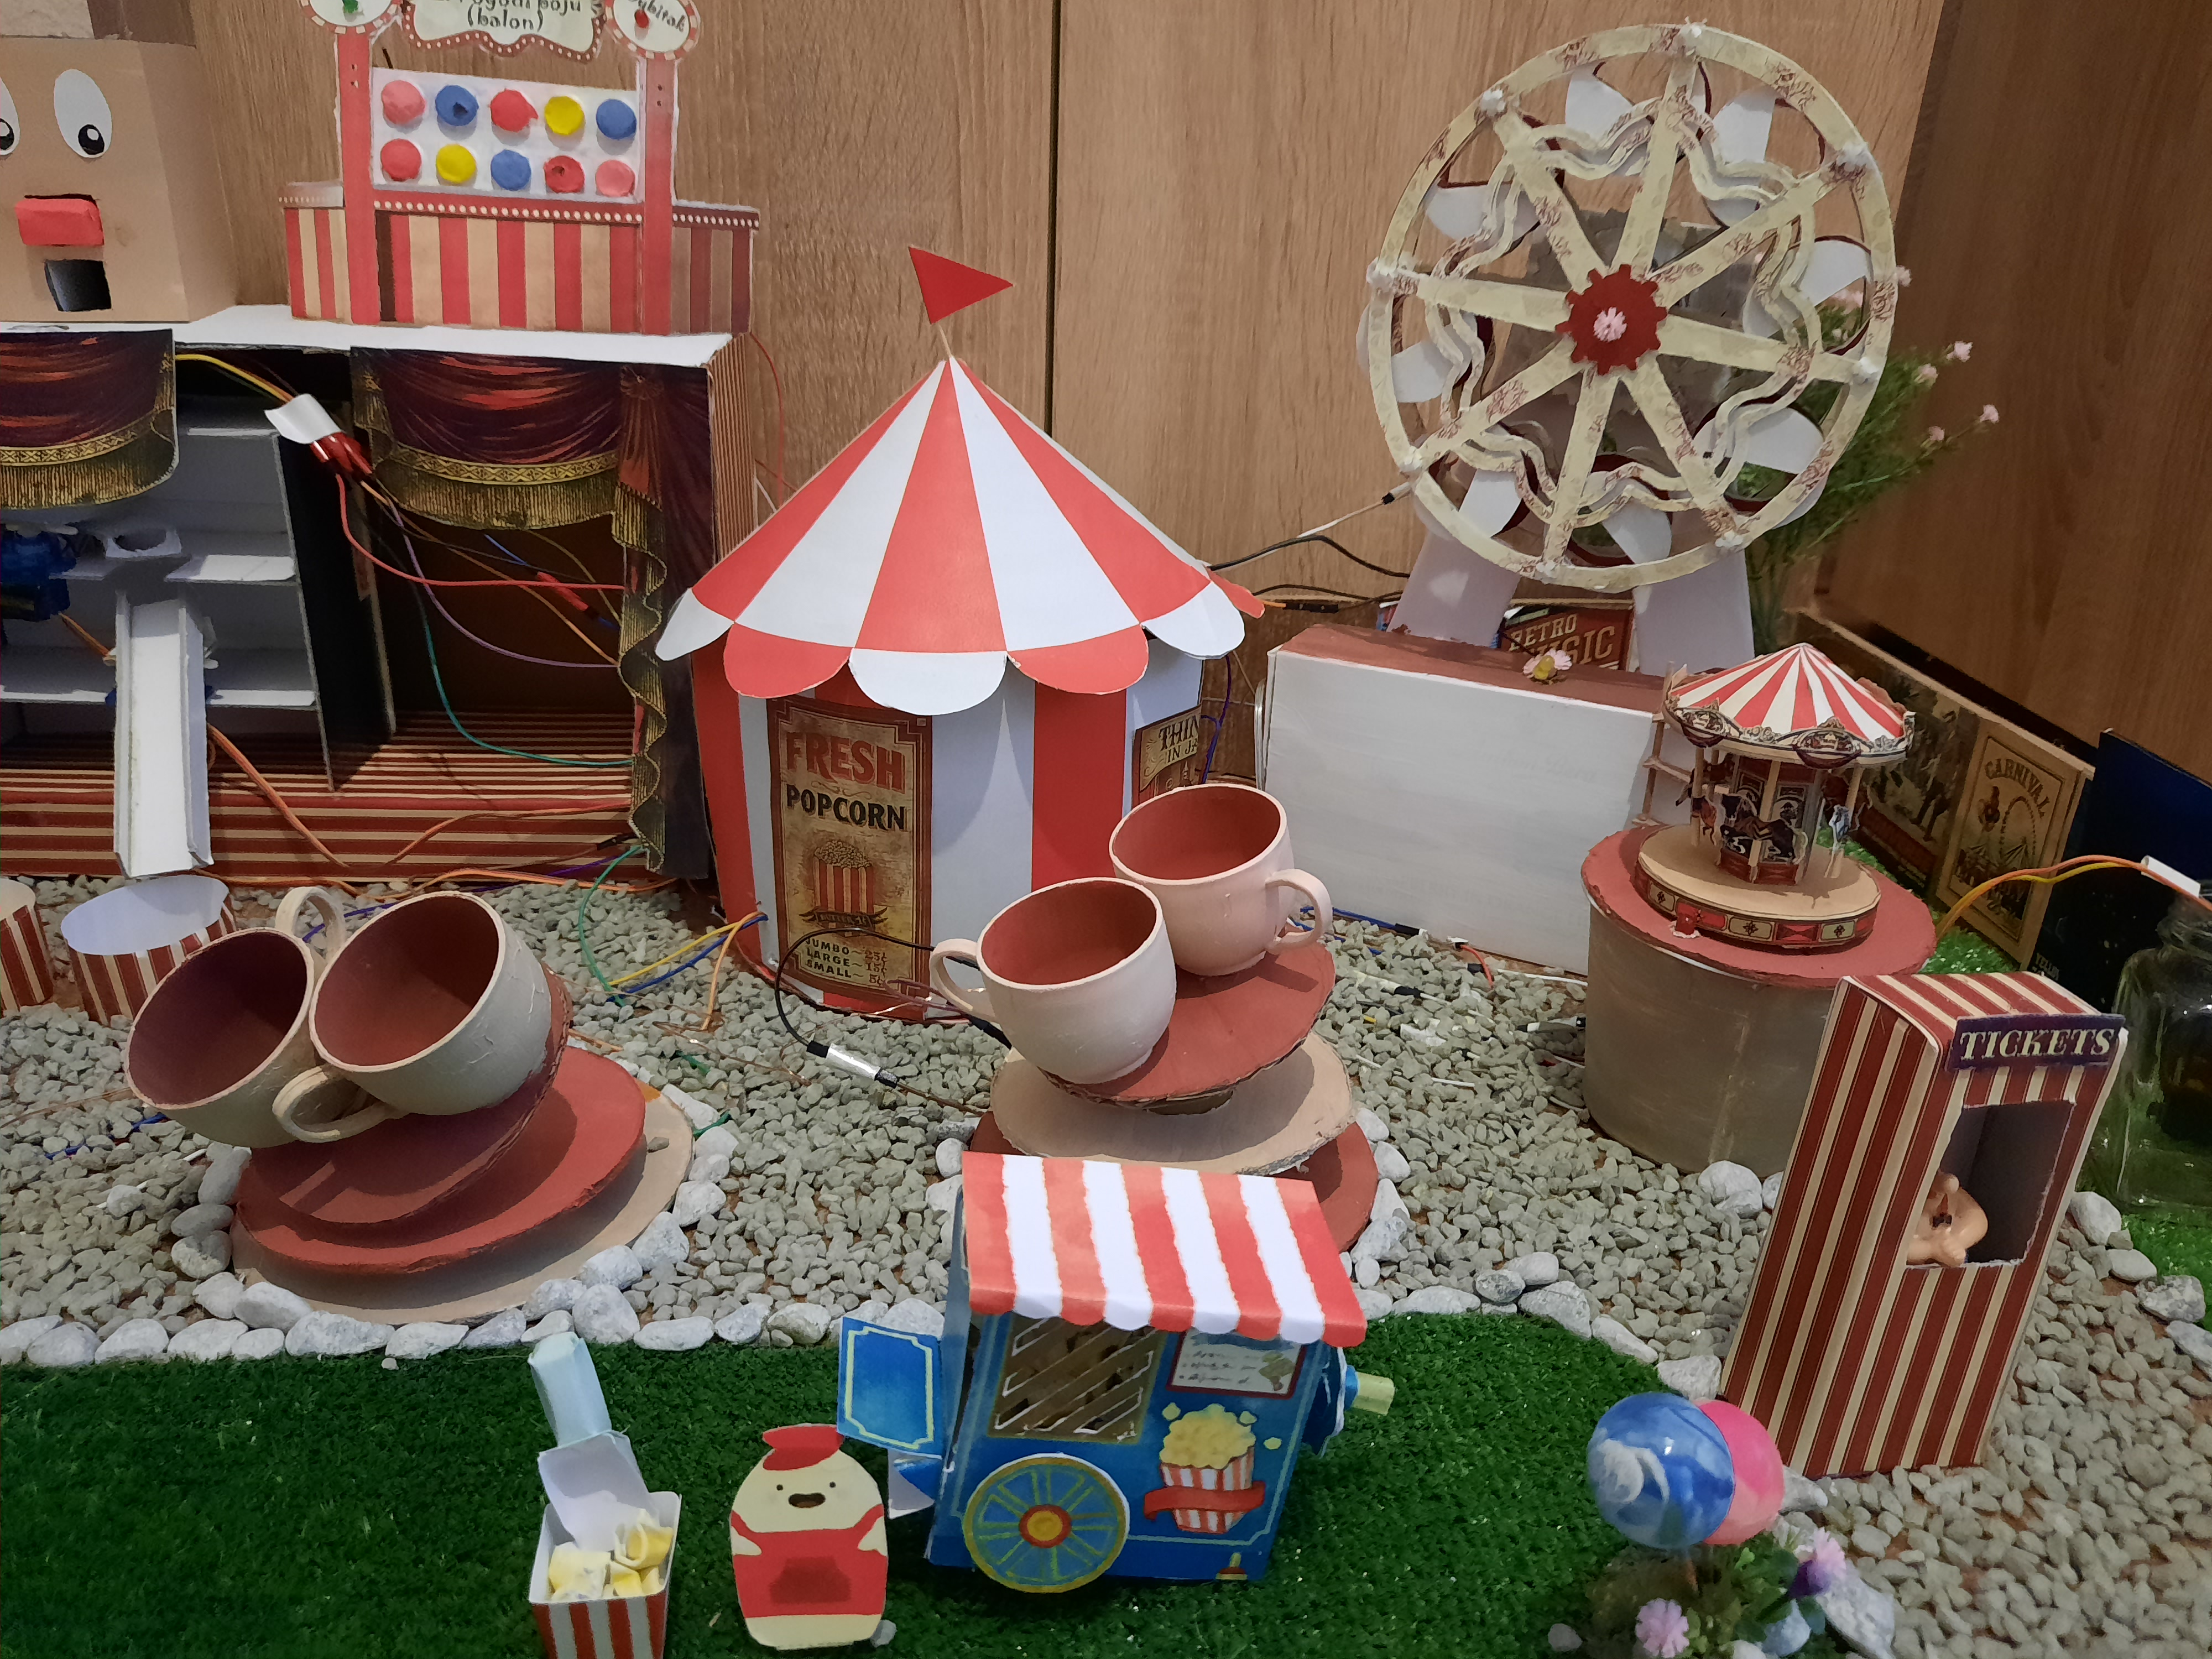
\includegraphics[width=0.7\textwidth]{pod2}
  \caption{Podsistemi  karusel, vrtuljak i šoljice}
  \label{fig:Slika_pod2}
\end{figure}

Sedmi podsistem je muzika koja se pušta s SD kartice preko zvučnika. SD kartica je morala biti povezana na posljednja 4 pina Arduino Mega pločice (prije 5 V pinova), pošto su to pinovi namijenjeni za asinhronu komunikaciju u kojoj je Arduino Mega pločica master element. Zvučnik je morao biti povezan na pin 5, 11 ili 46, inače ne bi radio. Pjesma za puštanje morala je biti konvertovana u .wav datoteku, sa frekvencijom 16 KHz, da bi zvuk bio neometano pušten. Pjesma se pokreće i zaustavlja po korisnikovoj želji uz pomoć aplikacije.

Svaki dio sistema prvotno je zasebno testiran, odnosno, sistem je rađen postepeno. Tek u završnoj fazi projektovanja sistema, svi su dijelovi sklopljeni u jednu cjelinu i usklađen je međusoban rad svih njegovih komponenti.

Motori koji pokreću određene dijelove prvo su testirani spajanjem direktno na napon, a tek onda povezani na modul, te na Arduino. Možda najzahtjevniji dio projektovanja sistema je bio usklađivanje napajanja, brzine vrtnje motora, te težine objekata koji se trebaju pokretati motorom. Kad je brzina motora premalena ili napon previše nizak, dijelovi se ne mogu vrtjeti, a prevelika brzina može oštetiti neki dio. Također, L298N driver za motore, jedini na lokalnom tržištu, nije savršen.

Rad sistema je jako teško prikazati na jednoj slici, puno bolji način je animacija ili video, s obzirom da se većina komponenti vrti, svijetli ili okreće, te se muzika sluša. 

 \begin{figure}[h!]
  \centering
  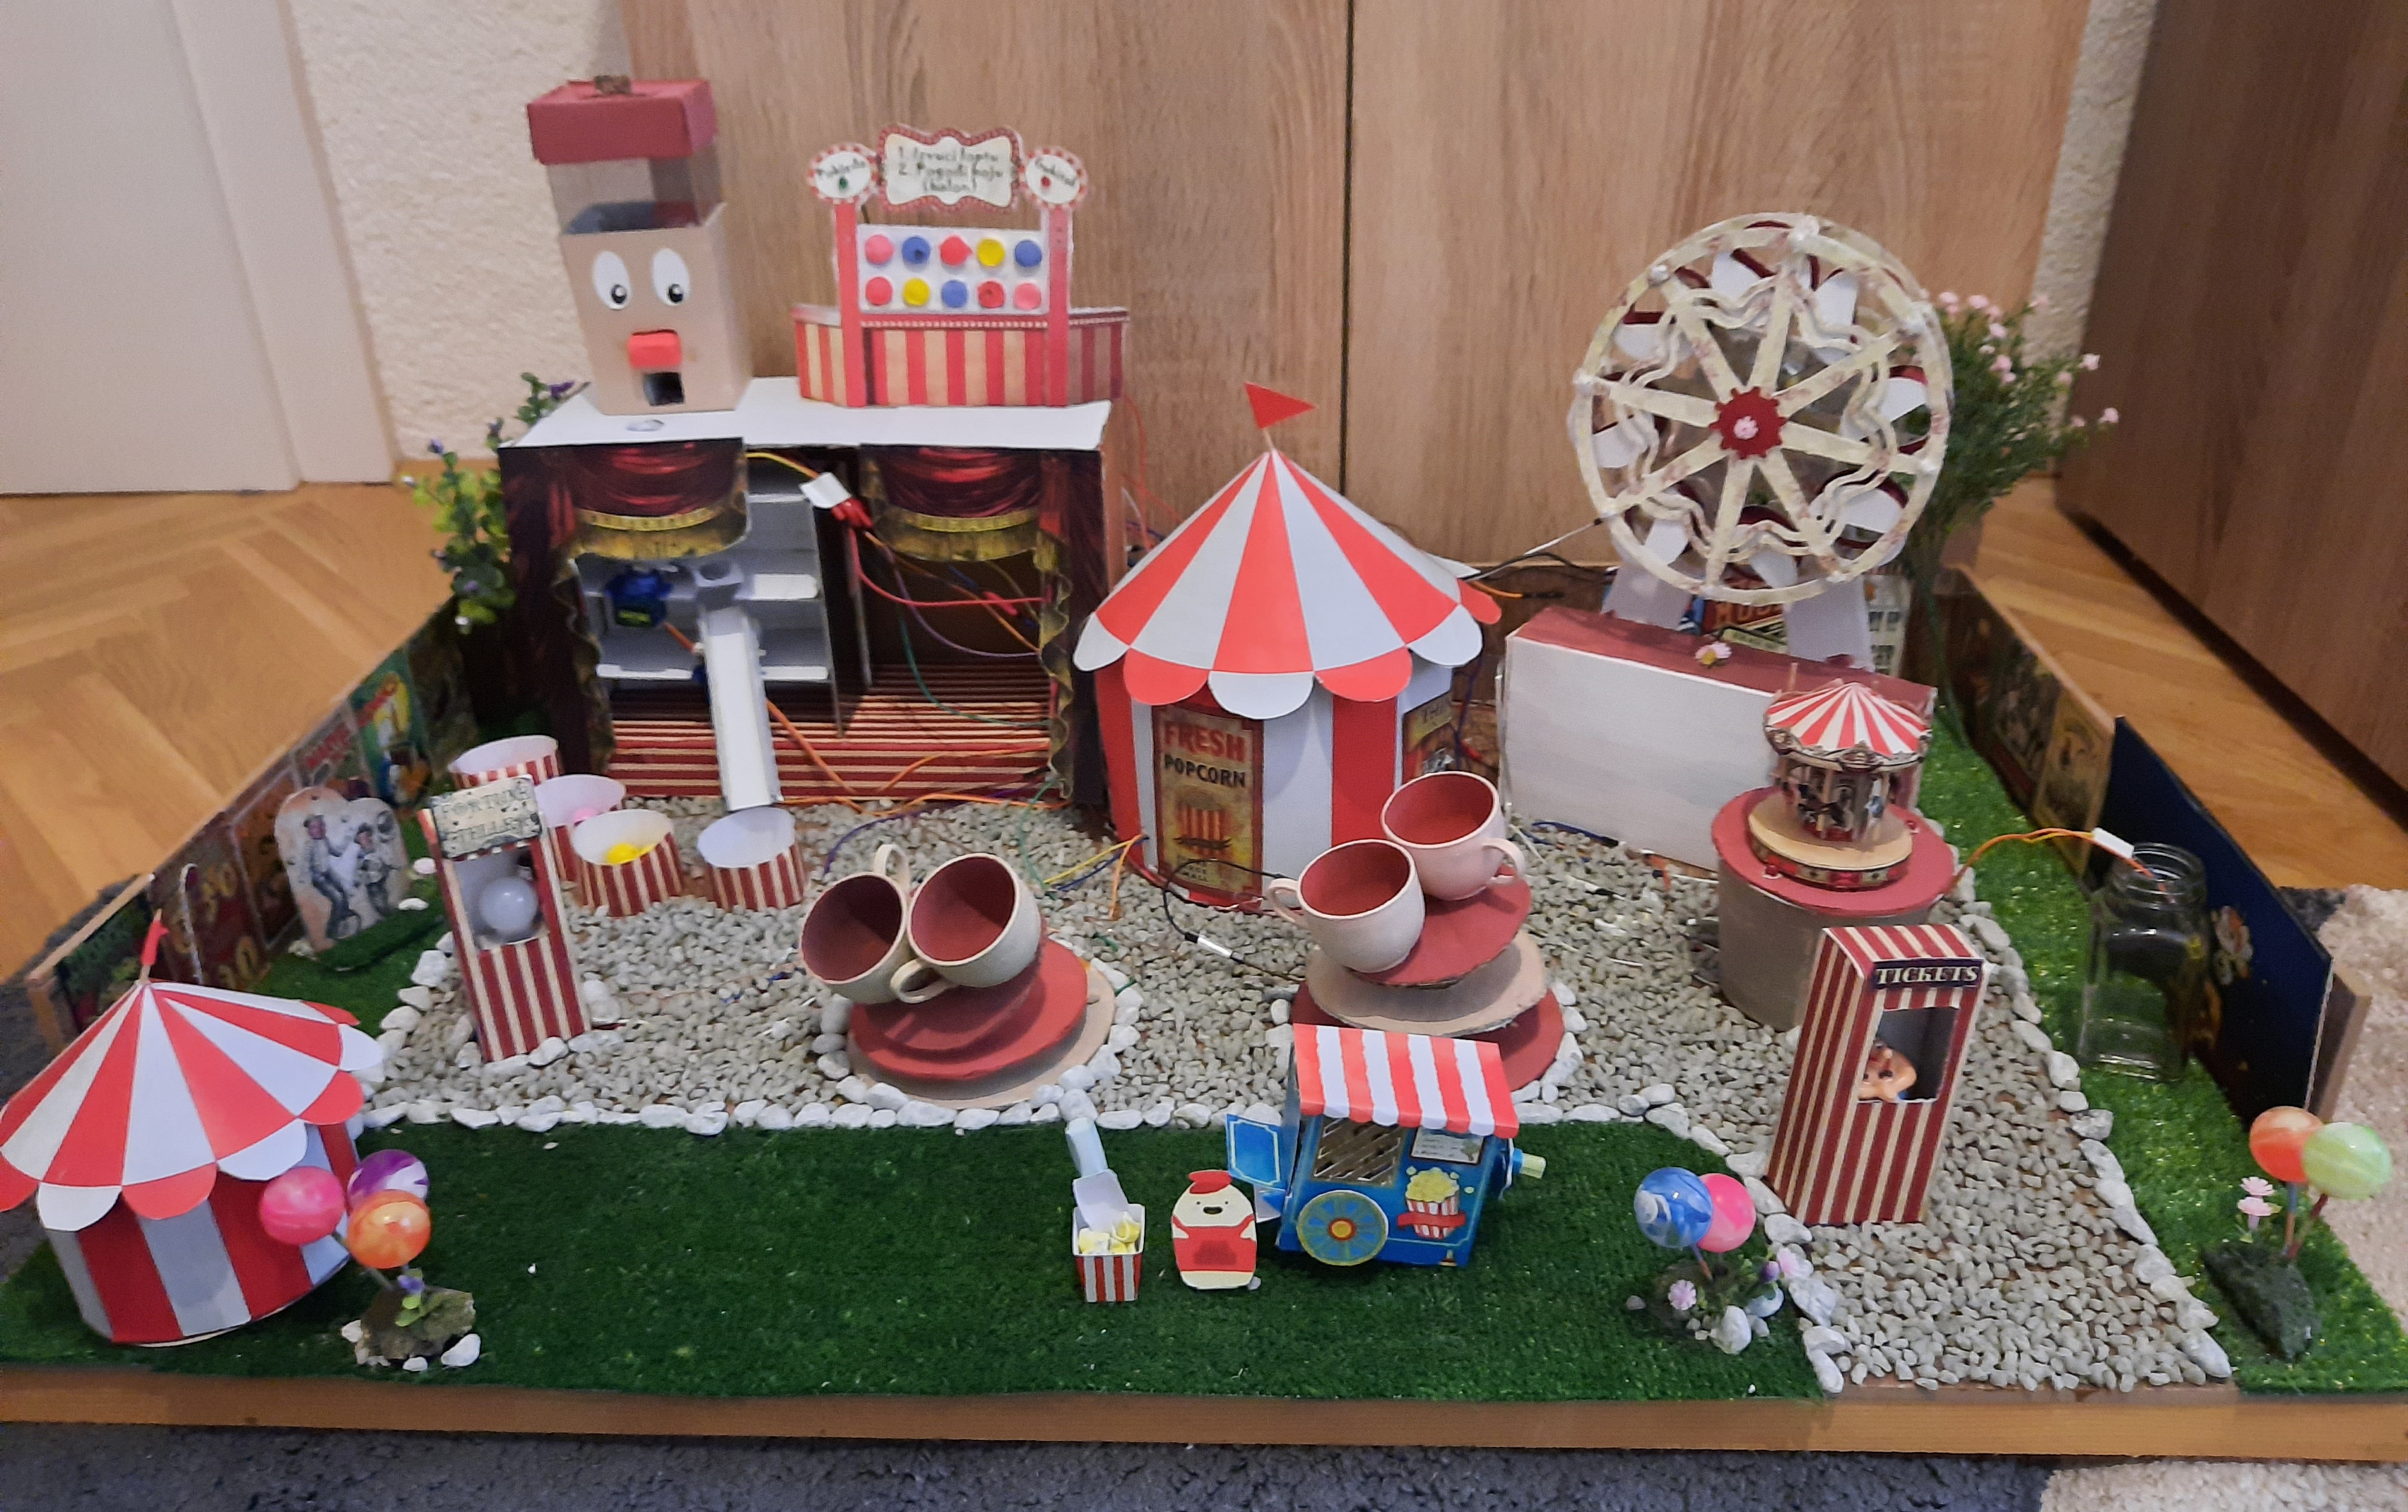
\includegraphics[width=0.7\textwidth]{maketa3}
  \caption{Maketa sistema}
  \label{fig:Slika_Maketa}
\end{figure}

Prednosti ovog sistema su da je potpuno jedinstven, stabilan, detaljan, te, zbog pozicioniranja USB kabla od Arduino pločice na lagano dohvatljivo mjesto, podložan nadogradnji i promjeni. Mane sistema su materijal, karton nije dobar materijal za gradnju, te nesavršenost komponenti.
